%%%%%%%%%%%%%%%%%%%%%%%%%%%%%%%%%%%%%%%%%%%%%%%%%%%%%%%%%%%%%%%%%%%%%%%%%
%
%	LaTeX File for Stanford University PhD Thesis
%
%%%%%%%%%%%%%%%%%%%%%%%%%%%%%%%%%%%%%%%%%%%%%%%%%%%%%%%%%%%%%%%%%%%%%%%%%
%	Copyright 2001  by  Jung-Suk Goo    (goojs@gloworm.stanford.edu)
%%%%%%%%%%%%%%%%%%%%%%%%%%%%%%%%%%%%%%%%%%%%%%%%%%%%%%%%%%%%%%%%%%%%%%%%%

\chapter{Introduction}

%%%%%%%%%%%%%%%%%%%%%%%%%%%%%%%%%%%%%%%%%%%%%%%%%%%%%%%%%%%%%%%%%%%%%%%%
%\section{Introduction} 
% allow  = 	permit, let, authorize, grant, empower, enable, entitle, qualify, agrees, offer, provide, express, show, assign, allocate, produce, construct, create, generate, induce, instigate, promote

% consistent = steady, stable, constant, regular, even, uniform, orderly, unchanging, unvarying, unswerving, undeviating, unwavering, unfluctuating, homogeneous, true to type; dependable, reliable, unfailing, predictable, reliable

% detect = 	identify, distinguish, establish, deduce, determine, differentiate, discriminate, discern, separate, characterise, discover, uncover, find, find out, turn up,  expose, reveal

% use = utilize, make use of, avail oneself of, employ, work, operate, wield, ply, apply, manoeuvre, manipulate,

%% In the introduction - do not explain any methods that are central to the comparison study
% Why Should we care?
%Background on group analysis - define group and explain, why are group interesting?
%
%1. Background.
%In this part you have to make clear what the context is. Ideally, you should give an idea of the state-of-the art of the field the report is about. But keep it short: in my opinion this part should be less than a page long. 
%Application motivation

%At the close of 2012, the monetary value of the world stock market was about US\$55 trillion.
Pointwise anomaly and change detection focus on the study of individual data instances that do not conform with the expected pattern in a dataset. With the increasing availability of multifaceted information, there is a growing trend in research involving groups or collections of observations. For example,  
 Muandet et al.	\cite{OCSMM} possibly detect Higgs bosons as a group of collision events  in high energy particle physics while a group of multiple sensor networks in Chen and Yu \cite{chen2016collaborative}, allow for a robust  detection of  distributed denial-of-service attacks. Group deviation detection  techniques achieve fewer false positives than pointwise approaches as a greater number of observations occur in group applications. %provide a better characterization of group behaviors. 
  Many pointwise anomaly detection methods are also not compatible  in detecting  group deviations so we turn to more specialized techniques.  
 



 

Group deviation detection involves the discovery of group behaviors which significantly deviate from the expected group patterns.   In particular, group anomaly detection (GAD) is the process of identifying groups that are not consistent with regular group patterns while group change detection (GCD) estimates significant deviations in the state of a group over  time. GAD and GCD methods achieve a higher performance  than pointwise methods for detecting group deviations. Even though GAD usually involves time-independent  applications and GCD relates to time-dependent groups, both problems share a common framework  and similar fundamental ideas.  
This survey  elaborates on group deviation detection techniques in static and dynamic situations. 

%Groups are also synonymous with collections, clusters or communities. 
%The terms group anomalies  and group outliers are interchangeable however we use group anomalies or anomalous groups in this survey.
 
% are synonymous with group outliers but  are also a specific type of collective contextual anomalies.    %Groups are defined according to different  contexts  where a group is a cluster of galexies in an astronomical dataset %\cite{OCSMM} ,MGM,FGM,GLAD}.
  %Group anomaly detection is the process of discovering patterns in groups that are not consistent with the expected behavior \cite{Chandola}. 

% emerging area of research


%Imagine a series of events leads to a financial butterfly effect and many portfolios of  stocks in the market require immediate asset reallocation. 


%groups exhibiting irregular behavior may represent a disease outbreaks  to malicious web spammers.  

  

%	  politics \cite{GLAD} 
  %Images in a photo album & Distortion \\

 
 
%Many papers mainly analyze the static natures of groups, however it is also interesting to monitor the evolution of groups over time. This is where multivariate time series and changepoint detection are applied.

% Group Distribution
%In our study, we focus on group behaviors based on numerical data. 




% \subsection{Definition of Groups} %
A group is a collection of two or more related data instances.    %F\~{a}rber et al. \cite{ClusterEval} even discusses how known group labels may not correspond to inherently clustered points. 
In GAD, a group anomaly has  significantly different  statistical properties  with respect to multiple groups whereas GCD involves detecting  a significant change   in a group  with respect to past group observations.   Group structures may be known a priori such as words in a documents otherwise when group   memberships between instances in a dataset are unknown, additional information or clustering algorithms are required. 
  Thus the initial definition of groups affects subsequent analysis and results. 
  %The validity of interpretations of known group labels and inherent clusters is discussed in  .   



 
    
   
More specifically,  Xiong et al.  \cite{MGM} categorize group deviations as either point-based or distribution-based for GAD applications.   Point-based anomalous groups are where all of the members are also pointwise anomalies. Similarly in GCD, a point-based group change signifies that time series in a group over time also experience significant changes.   On the other hand, a  distribution-based group anomaly  is where a collection of points differs from expected group patterns, however individual data instances may not seem anomalous. Likewise, a distribution-based change in a group over time occurs when individual time series exhibit regular behavior however their collective pattern is significantly different.   

 % between multiple variables. 
  
%  %  groups are represented by a set of features. %descriptive properties. 
%One way of specifying features of a group is through statistical properties of group distributions  such as location, scale, shape and dependence between multiple variables.   %Other  descriptive properties of a group % distributions 
%Other descriptions of group features such as rules and network connections are dependent on the availability of data. 
 
 

  %Their study investigates examples of Gaussian mixtures where a group anomaly is generated from a different proportion of distributions. 

%In these cases,  individual data instances exhibit regular behavior however the collective behaviors of roup 3 are anomalous in Figure \ref{Fig:Intro}. Since there are a variety of statistical properties for a group distribution, it is difficult to robustly capture anomalous behaviors using pointwise anomaly detection methods.





 %We focus on measures of distributions in terms of location, scale, shape and dependence between multiple variables. Different detection techniques have a better performance for particular anomalous patterns. 
  %  Thus our research analyzes a variety of  statistical properties as described in Table \ref{Tab:Des}. Most group anomaly detection methods are interested in distribution-based anomalies which are 




%\begin{figure}[H]
%\centering
% \begin{subfigure}[b]{0.6\textwidth}
%                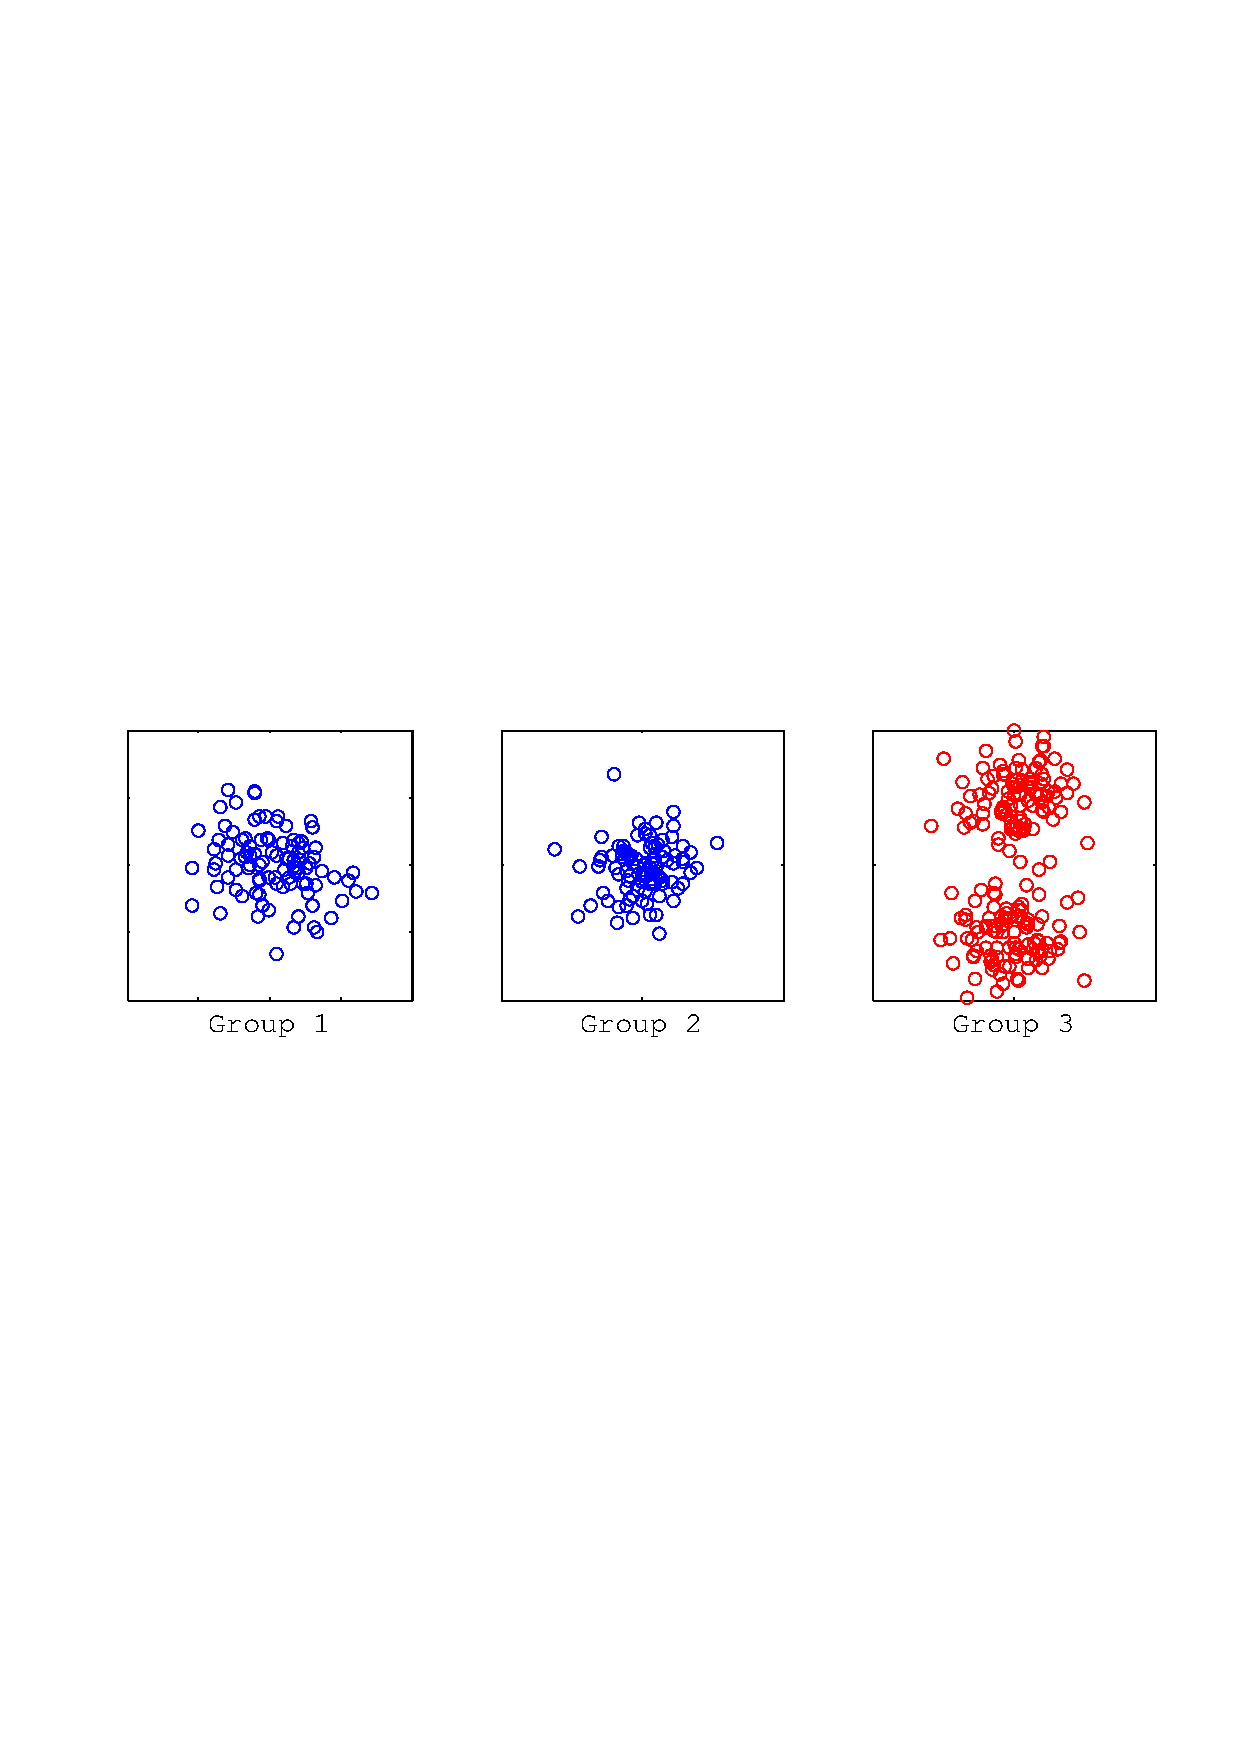
\includegraphics[width=\linewidth,trim=3cm 12cm 3cm 11.5cm]{Ex1}
%                \caption{A significant deviation in scale or shape.}
%        \end{subfigure}%
%        \hfill
% \begin{subfigure}[b]{0.6\textwidth}
%                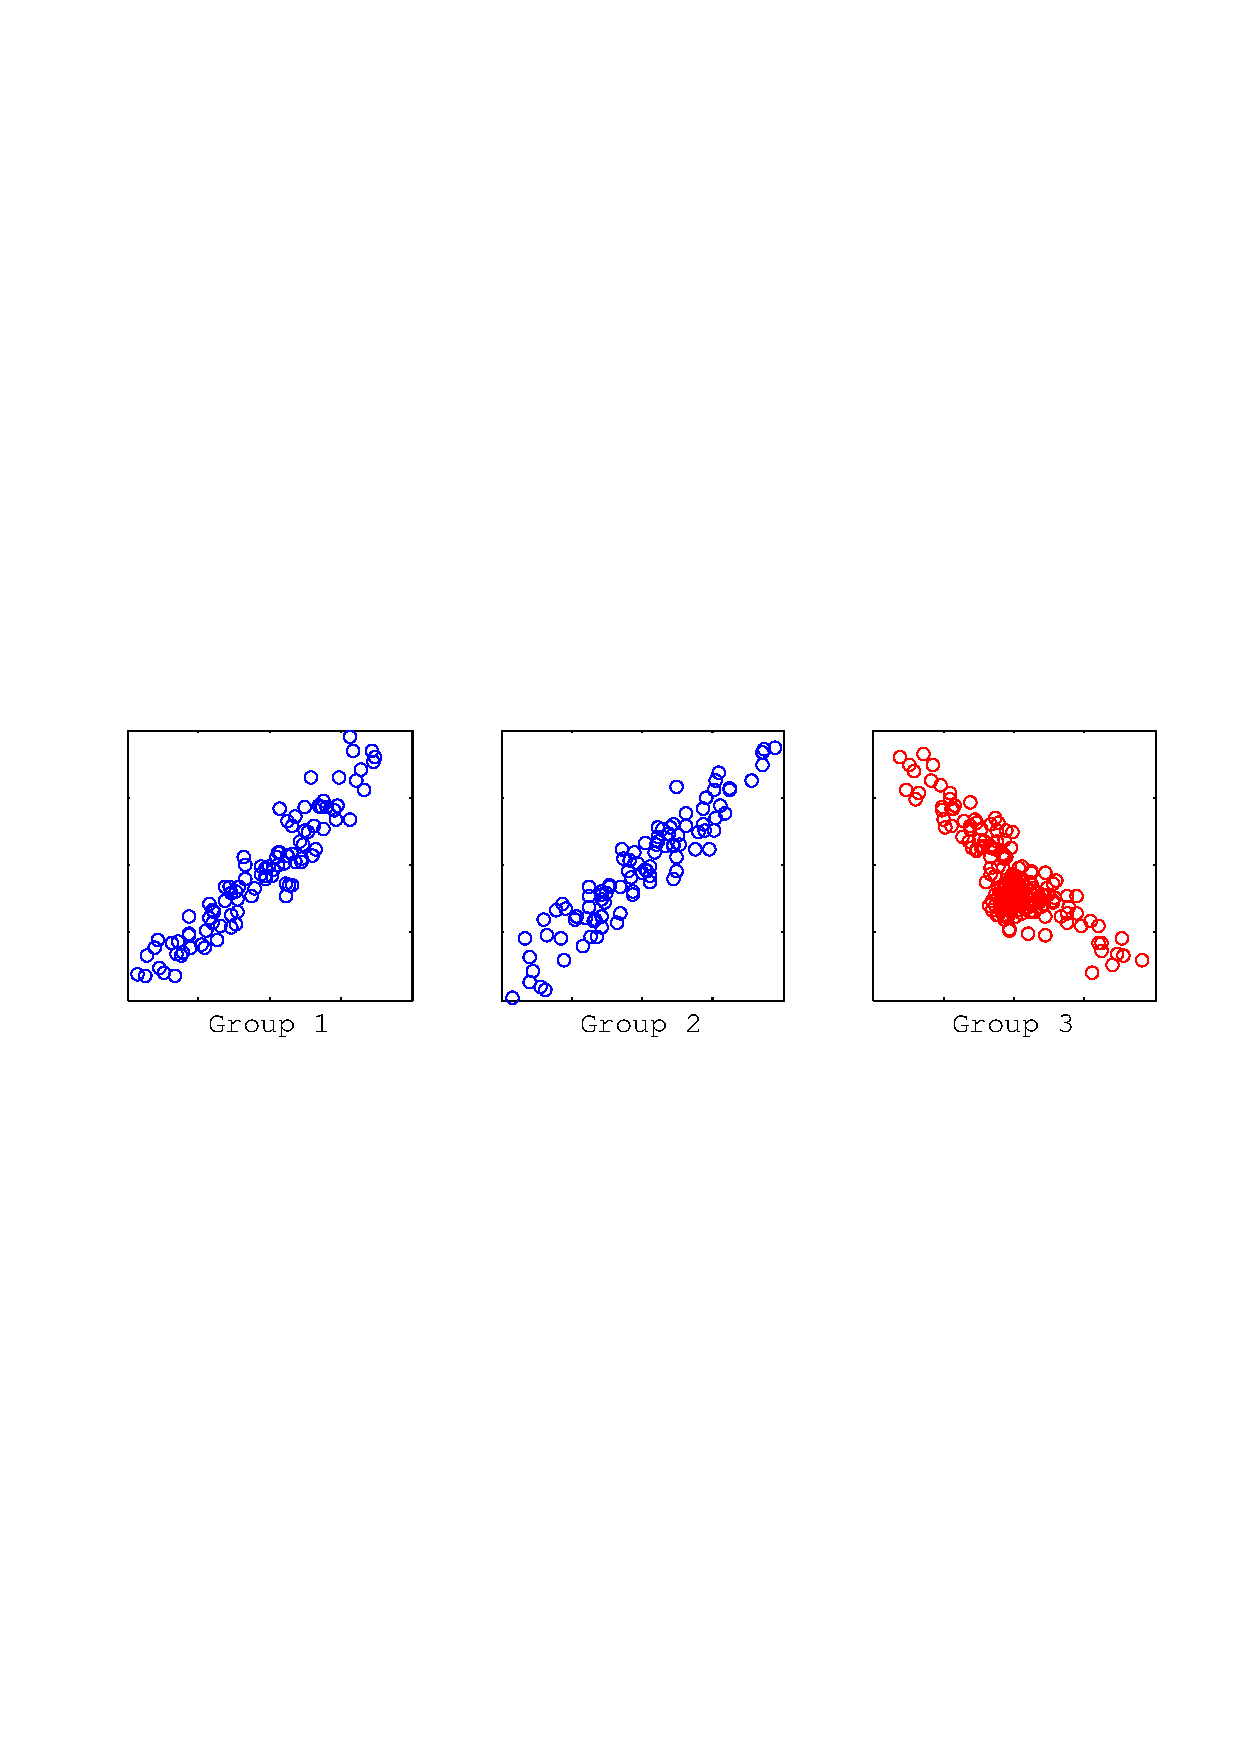
\includegraphics[width=\linewidth,trim=3cm 12cm 3cm 11.5cm]{Ex2}
%                \caption{Significant deviation in covariance or correlation. }
%  \end{subfigure}%
%%\includegraphics[width=7.5cm, height=5.2cm,trim=3cm 9cm 3cm 10cm]{ToyExample}
%\caption{Examples of group behaviors that clearly deviate in terms of different statistical properties; (a) scale or shape and (b) covariance or correlation.  
%}
%\label{Fig:Intro}
%\end{figure} 


 Figure \ref{Fig:Intro} highlights two examples where distribution-based group deviations are characterized by two different statistical properties. The first row in (a) illustrates Group 3 with a relatively greater  scale or shape whereas in the second row (b),  a Group 3 is characterized by a rotated covariance or correlation structure between variables. 
 % Depending on the context, Group 3 in each row of Figure \ref{Fig:Intro} may represent   a group anomaly for a GAD application whereas in a GCD context, Group 3 is a time-dependent group where a significant change in group occurs at $t=3$.  
  {  
  Depending on the specific domain, the group deviation (Group 3) in  Figure \ref{Fig:Intro} has different interpretations. In Xiong et al. \cite{MGM}, a group anomaly represents an anomalous galaxy with a significantly different scale or shape parameter whereas Chen et al. \cite{GLETS}  examine a GCD context where a significant deviation in correlation between stocks occurs over time.     
    }

%\subsection{Applications}
%By considering a group rather than an individual instance is  beneficial in a diverse range of applications.
 GAD and GCD  techniques provide meaningful insights that are not effectively detected by pointwise  methods  in a diverse range of applications.  
In intrusion detection,  Chen and Yu \cite{chen2016collaborative} explore  a collaborative detection system involving multiple sensor networks to detect distributed denial-of-service attacks. Using collective information from multiple intrusion detection system rather than a single system offers a more reliable detection of coordinated attacks. Another example is where Dai et al. \cite{ERACD} analyze an IMDb movie database where anomalous collection of entities contain highly ranked actors that are otherwise not discovered by pointwise detection methods.   Real-world GAD events have also been studied in group psychology such as  high  performance of employee work teams by   Kozlowski and Bell  \cite{kozlowski2003}.  
   %Zhou et al. \cite{Zhou2010}  A Survey of Coordinated Attacks and Collaborative Intrusion Detection}

Investigating group deviations has a variety of interesting domains, especially physical GAD applications.  %that motivate different avenues of research.
In particular,  Muandet et al.	\cite{OCSMM} investigate GAD for physical phenomena in high energy particle physics such as Higgs bosons that are observed as slight excesses in a collection of collision events rather than individual  events. In Guevara et al. \cite{SMDD}, an anomalous galaxy cluster is identified by an irregular proportion of color pixels. Xiong et al. \cite{FGM} also analyze a physical application with 3-dimensional velocity of a fluid from the  JHU turbulence database  
where a group anomaly represents unusual vorticity in  fluid dynamics.  
 

Textual data is also examined in GAD where a document is considered a group of words. 
Yu et al. \cite{GLAD} investigate scientific publications in order to understand the structure of certain research communities. Irregular communities of co-authors possibly reveal unusual research trends.  By analyzing documents from a training set of news articles, Soleimani and Miller \cite{ATD} infer regular topics   such as $`\mathtt{rec.sport.baseball}'$  and $`\mathtt{ talk.politics.misc}'$. An anomalous cluster in this case consists of novel topics that are unobserved in the training corpus such as $`\mathtt{rec.sport.hockey}'$ and $`\mathtt{talk.politics.mideast}'$. Using  textual information from product reviews on Amazon, Mukherjee et al.  \cite{GroupReviewSpam} identify  groups of spammers that collaborative in writing fake reviews. 

%There are many other applications where GAD and GCD techniques offer interesting results. 
  
  A group over time for GCD is also studied across a variety of domains.  Wong et al. \cite{wong-rule} investigate different demographic groups admitted to  emergency departments in hospitals in a major US city.   A significant change in a particular demographic group over time represents an early indication of a potential epidemic and disease outbreak. 
  Chen et al. \cite{GLETS} monitor a group of  time series  in the stock market where after a specific period, the group disbands with dissimilar individual behaviors.     In this case, a group of seemingly uncorrelated time series may also form a more cohesive collection with a higher correlation over time.  Using multiple sensor data, Xie and Siegmund  \cite{xie2013} explore a general problem of sequential change detection in a proportion of time series in a group over time.   In a political application, Yu et al. \cite{GLAD} discover  a large deviation in voting behaviors of a group of US senators around the time of a Democratic party  election.  
  A real-world GCD event has been discovered in five of the largest private health insurers in Chile where they colluded to unfairly reduced  the coverage of healthcare plans over a period of time \cite{Chile}.  

%Thus once a group anomaly is discovered,  an actionable intervention depending on the particular domain may lead to  mitigating health  risks to reduction of unfair monetary losses. 
 Thus there are interesting and meaningful insights that are gained from GAD and GCD applications such as: 
\begin{enumerate}
\item  New research discoveries; 
Higgs bosons in physics \cite{OCSMM}, 
 anomalous galaxy clusters in astronomy  \cite{SMDD},  unusual vorticity in fluid dynamics \cite{FGM}. 
\item  Mitigation of risks: reduce financial losses  \cite{GLETS}, prevent disease outbreaks  \cite{wong-rule}.
\item   Identification of  fraudulent collaborative  activities:  collusion detection \cite{Chile}, fake product reviews on Amazon  \cite{GroupReviewSpam}, % identifies collaborative group of spammers that write .
 intrusion detection for  distributed denial-of-service attacks  \cite{chen2016collaborative}.   
\item  Interesting  explanatory results;   research trends in academic communities   \cite{GLAD},  changes in political voting preferences \cite{GLAD},  
highly ranked actors in IMDb movies   \cite{ERACD}, performance of employee work teams  \cite{kozlowski2003}.  
\end{enumerate}  

   % Table \ref{Tab:Examples} summarizes group applications explored in the literature and provide a basic interpretations of their results.   
   
% 		\begin{table}[H]
%	\tabcolsep=0.2cm  	\renewcommand{\arraystretch}{1.8}
%	\begin{center}
%	\scalebox{0.8}{
%	\begin{tabular}{|p{3.5cm}|c|l|l|l|l }
%	\hline\\[-5mm]
%%Techniques &	
%Authors & \small Application & Group Dataset & Interpretation of  Results %Group Anomalies
%  \\ \hline \\[-5mm] 
%	% Molecular biology  & Irregular protein-protein interaction \cite{MMSB} \\
%%Discriminative Model  & 	
% \small Chen and Yu \cite{chen2016collaborative}&   & Collaborative  Intrusion Detection % System
%    &
%  Distributed denial-of-service   \\
% Muandet et al.	\cite{OCSMM} &   & High Energy Particle Physics  & Signals  containing  Higgs bosons  \\
% Guevara et al.	\cite{SMDD} &  & Sloan Digital Sky Survey  & Irregular cluster of galaxies  \\
%%\hline\\[-6mm] 
%%\small Xiong et al. \cite{MGM}  &	 Sloan Digital Sky Survey & Irregular cluster of galaxies  \\
%% 	\small Xiong et al. \cite{FGM} & Generative Model &
%% Generative Model  &
%\small Xiong et al. \cite{FGM} & GAD & JHU Turbulence Database Cluster  & Unusual vorticity \\%Image of Fluid Motion   & Unusual turbulence   \\ % Image Data  & Stitched images from different scenes  \\
%	\small Yu et al. \cite{GLAD} &  & Scientific Publications & Research trends in communities  \\
%Mukherjee et al.  \cite{GroupReviewSpam} &  &  Amazon reviews  & Groups of manipulative spammers \\ 
% \small Soleimani and Miller \cite{ATD}  &  & 20-Newsgroup Dataset  & Anomalous document collection   
% \\
% 	\small Dai et al. \cite{ERACD} &  &
%	IMDb Movie Database & Highly ranked actors  
%  \\   
%%Kozlowski et al. \cite{kozlowski2003}  
%\hline 
%	\small Yu et al. \cite{GLAD} &  & Political Voting & Changing voting preferences \\
%  \small Wong et al. \cite{wong-rule} 
%& \multirow{2}{*}{GCD} & Emergency Department %Database 
%	 &  Disease outbreaks \\
%     \small Chen et al. \cite{}  &   &  Stock Market Data     & Increased market variability   \\
%  Xie and Siegmund  \cite{xie2013} &   & Sequential Sensor Data & Change detection  in multiple sensors    \\ 
%     [2mm]
%   %Detecting Extreme Rank Anomalous Collections 
%% %Web Host Graph & Web Spammer entities \\
%% 
% \hline
%	 \end{tabular}
%	 }
%	 \smallskip
%	\end{center}
%	 with interpretations of group devi\caption{ Previous studies involving GAD and GCD applicationsations. }
%\label{Tab:Examples}
%\end{table}   


{ 
%\subsection{Our Contributions}
The objective of this survey paper is to provide a clearer understanding and detailed  overview of group deviation detection research.  %anomaly and change detection techniques involving group observations.  
 We first explain GAD techniques  in multiple static groups and then explore dynamic groups for GCD applications. %We also provide an evaluation of each procedure and suggest future research directions where techniques can be further improved. % Since some methods are  specifically design for a particular domain, we elaborate on the different applications for group anomaly detection.
Our  main contributions are  summarized as: %\vspace{-1mm}
\begin{enumerate}
\item {\bf Clearer Understanding:} 
This survey provides an underlying structure for   both group anomaly detection (GAD) and group change detection (GCD) problems.      % Figure \ref{Fig:Framework}  builds upon the anomaly detection from Chandola \cite{Chandola}
\item {\bf Detailed Overview:} 
 We further elucidate the details of state-of-the-art techniques in terms of four key components as described in Section \ref{Sec:Problem}. 
\item {\bf Discussion:} We also discuss the advantages and disadvantages of current GAD and GCD techniques in terms of discriminative methods, generative models  as well as hypothesis tests. 
\end{enumerate}
 
%\section{Organisation}
The rest of the paper is organized as follows. Section \ref{Sec:Framework} describes the underlying structure and ideas relating to group deviation detection.  Section \ref{Sec:Problem}  formalizes the group deviation detection problem where techniques are explained in terms of four key components. Techniques for detecting group anomalies are explained in Section  \ref{Sec:D} while Section \ref{Sec:GCD}  describes methods for detecting significant changes in a group over time. A discussion of our findings and future research for group deviation detection is provided in Section 
 \ref{Sec:Discussion} while Section \ref{Sec:Conclusion} summarizes our survey paper.
}
 